% Draft for ICML 2027. The official icml2027.sty is not out yet; this file uses a plain two-column
% layout of the same size. To switch: \usepackage{icml2027}, then the \icmltitle / \icmlauthor blocks.
\documentclass[10pt,twocolumn]{article}
\usepackage[letterpaper,top=1in,bottom=1in,left=0.75in,right=0.75in,columnsep=0.25in]{geometry}
\usepackage{times}
\usepackage[T1]{fontenc}
\usepackage{amsmath,amssymb}
\usepackage{booktabs}
\usepackage{graphicx}
\usepackage{xcolor}
\usepackage[numbers,sort&compress]{natbib}
\usepackage[hidelinks]{hyperref}
\usepackage{caption}
\captionsetup{font=small,labelfont=bf}

\newcommand{\todo}[1]{\textcolor{red}{[TODO: #1]}}
\newcommand{\Tlb}{T_{\mathrm{lb}}}
\newcommand{\Tref}{T_{\mathrm{ref}}}

\title{\Large\bf Where Does the Time Go When LLM Agents Work as a Team?\\
\large An Auditable Study of Scaling, Handoffs, and Self-Organized Crews}
\author{Anonymous Authors}
\date{}

\begin{document}
\maketitle

\begin{abstract}
Teams of language-model agents are often assumed to get faster as they grow, but it is rarely measured how far a team is from the best any team could do, or where the lost time goes.
We build a multi-agent environment in which a problem's total work and critical path are known exactly and cannot be shortcut by reasoning: a layered DAG of tasks, each of which can only be solved by evaluating a hidden keyed function one call at a time.
This gives every run a hard lower bound $\Tlb$ and lets us account for each lost round from the traces.
With teams of 1 to 32 identical agents and no prescribed organization, a frontier model reaches an 8.7$\times$ speed-up at 32 agents, but its efficiency against the bound falls from 0.98 alone to 0.49 at 16 agents.
The loss concentrates in two places: handing a layer's answers to the next (4--5 rounds per layer, 2--3$\times$ a scripted team) and the final join, which costs one extra round for every answer its solver pulls from the shared store.
When agents outnumber a layer's tasks, teams spontaneously split into two alternating crews that hide the handoff.
We registered four predictions before running them: two quantitative scaling laws failed, while two mechanistic predictions held on every seed, including an out-of-sample shape and an intervention that forbids the second crew.
\todo{one sentence on the open-weight replication (Qwen3) once the runs are in.}
\end{abstract}

\section{Introduction}

Multi-agent systems built from large language models (LLMs) now divide software projects, research pipelines and simulations among many agents \citep{wu2023autogen,hong2024metagpt,qian2024chatdev,chen2024agentverse,park2023generative}.
A natural question is how such a team scales: if one agent takes $T(1)$ to solve a problem, how long do $N$ agents take?
Recent work reports that adding agents helps on some tasks and hurts on others \citep{li2024moreagents,qian2025macnet,kim2025scaling}, and catalogues how multi-agent systems fail \citep{cemri2025fail}.
What is usually missing is a \emph{reference point}: without knowing the fastest any team could solve a problem, a speed-up of 5$\times$ cannot be read as good or bad, and the lost time cannot be located.

Parallel computing has had this reference point for fifty years.
For a computation with total work $W$ and critical path (span) $D$, no schedule on $N$ processors finishes in fewer than $\max(\lceil W/N \rceil, D)$ steps \citep{brent1974,graham1969}.
We build an environment where this bound holds exactly for LLM agents, and use it to ask three questions.
\textbf{(Q1)} How close do LLM teams come to the bound as they grow?
\textbf{(Q2)} Where, step by step, does the remaining time go?
\textbf{(Q3)} Do teams organize themselves to recover it, and can we show that causally?

\paragraph{Contributions.}
\begin{itemize}\setlength\itemsep{1pt}
\item \textbf{An environment with exact bounds.} Tasks are chains of a hidden keyed hash with no repeated value, laid out as a layered DAG (\S\ref{sec:env}). Reasoning cannot skip an evaluation, so total work and span are hard lower bounds for any strategy, and every accepted answer is audited call by call.
\item \textbf{A time decomposition.} Synchronous lockstep rounds make a team's time comparable with the bound and with scripted reference teams, and split it into per-layer handoff loss and join loss (\S\ref{sec:metrics}).
\item \textbf{Findings.} LLM teams parallelize (8.7$\times$ at 32 agents) but lose 2--3$\times$ more per handoff than scripted teams; the join costs one round per answer read from the store; and teams with spare agents form two crews that halve the handoff loss (\S\ref{sec:results}).
\item \textbf{Pre-registered tests.} All four predictions were written before their runs (\S\ref{sec:prereg}). We report the two that failed alongside the two that held, including an intervention that removes the second crew.
\end{itemize}

\section{Related Work}

\paragraph{LLM multi-agent systems.}
Frameworks organize agents by roles and conversation \citep{wu2023autogen,li2023camel}, by standard operating procedures \citep{hong2024metagpt,qian2024chatdev}, or by dynamic recruitment \citep{chen2024agentverse}; generative agents populate simulated towns \citep{park2023generative}; debate improves answers by aggregating agents \citep{du2024debate}.
Deployed hierarchical systems report that hierarchies must be designed by hand and that details are lost in message passing \citep{zou2025elagente}.
These works measure task success; we measure \emph{time against a bound} on a task whose success is fixed.

\paragraph{Scaling the number of agents.}
Sampling-and-voting scales with agent count on reasoning benchmarks \citep{li2024moreagents}; networks of hundreds of agents show a logistic quality curve \citep{qian2025macnet}; and controlled comparisons of single- and multi-agent architectures find that the benefit depends on the task's decomposability \citep{kim2025scaling}.
Failure taxonomies attribute many multi-agent failures to inter-agent misalignment \citep{cemri2025fail}.
Our environment makes decomposability a parameter (width, depth and grain) and gives the exact best case, so the cost of coordination can be measured in rounds.

\paragraph{Parallel performance models.}
Amdahl's law \citep{amdahl1967}, Brent's bound \citep{brent1974,graham1969}, bulk synchronous parallelism (BSP) \citep{valiant1990bsp} and the Universal Scalability Law (USL) \citep{gunther2007usl} describe how parallel programs scale. We test whether the last two predict LLM teams; neither does.

\section{Environment}
\label{sec:env}

\paragraph{The network.}
Agents act through a simulator that runs a task market, messaging, a public board and a versioned shared store, and charges every operation (Table~\ref{tab:ops}). It never says how agents should cooperate.

\begin{table}[t]
\centering\small
\caption{Operations available to every agent.}
\label{tab:ops}
\begin{tabular}{@{}ll@{}}
\toprule
operation & effect \\
\midrule
\texttt{tasks} & list open, blocked and done tasks \\
\texttt{apply} & evaluate a task's hidden function once \\
\texttt{submit} & hand in an integer answer, checked exactly \\
\texttt{send}, \texttt{inbox} & message other agents \\
\texttt{put}, \texttt{get}, \texttt{keys} & shared, versioned store \\
\texttt{wait} & pass one round \\
\bottomrule
\end{tabular}
\end{table}

\paragraph{The problem.}
A problem has \emph{depth} $d$ layers of \emph{width} $w$ tasks and one final task.
Each task $T$ owns a hidden function $f_T:\{0,\dots,999\}\to\{0,\dots,999\}$, a keyed BLAKE2 hash.
A layer-0 task starts from a given number; a later task starts from the sum, mod 1000, of the answers of two random tasks in the layer before; the final task starts from the sum of the whole last layer.
A task's answer is $f_T$ applied \emph{grain} $g$ times in a row, and the only way to evaluate $f_T$ is one \texttt{apply} call per value.
The key is chosen so that no chain repeats a value, so no earlier output can stand in for a call.

\paragraph{Bounds.}
Solving a task costs exactly $g$ applies and one submission, and it cannot start before its parents are known. With $n_T = wd+1$ tasks, total work is $W = n_T(g+1)$ actions and the span is $D = (d+1)(g+1)$, so a team of $N$ needs at least
\begin{equation}
\Tlb(N) = \max\left(\lceil W/N \rceil,\; D\right)
\end{equation}
rounds \citep{brent1974}. This holds for any strategy, however capable the model.
An earlier version based on symbolic recurrences did not have this property: a strong model wrote the whole DAG as one closed-form expression without calling a tool. We report it as a negative result in Appendix~\ref{app:history}.

\paragraph{Teams.}
In the \texttt{peers} design, $N$ identical agents start together with the same tools, the same briefing and an equal share of the call budget. They are told only that they are $N$ identical agents working on one problem and should share the work as they see fit. There is no orchestrator or role. With $N=1$, the same design is a single agent, so speed-ups compare like with like.

\paragraph{Time.}
LLM agents run at different speeds, so wall-clock time mixes model latency with coordination.
We use \emph{lockstep} rounds instead: in each round, every agent still working chooses one action, and the actions are then applied in a fixed order.
A slow member therefore holds up the team, as a slow processor would.
$T$ is the round in which the final task is accepted.

\section{Metrics}
\label{sec:metrics}

\textbf{Speed-up} is $T(1)/T(N)$; \textbf{efficiency} is $b = \Tlb/T \le 1$.
As a practical reference, $\Tref$ is the fastest of three scripted teams that broadcast each answer, share a store, or batch a layer's answers.

\paragraph{Where the time goes.}
For each layer $\ell \ge 1$ we compute the \emph{handoff loss}: the rounds the layer took beyond the fastest it could go, given when its inputs became available. The \emph{join loss} is the same quantity for the final task.
Layer 0 has no handoff and is excluded.
Both are computed from the traces, which also record every store read, message and claim.

\paragraph{Audit.}
For every accepted answer we check its complete apply chain, its parents and its integer value. Across all runs reported here, every accepted node passed.

\section{Results}
\label{sec:results}

\paragraph{Setup.}
The main problem is $w=16$, $d=4$ (65 tasks) at grain $g\in\{1,4\}$, with $N\in\{1,2,4,8,16,32\}$ and seeds 100--102.
The model is a closed frontier model (\texttt{gpt-6.1-sol}, high reasoning effort) driven through its agent CLI.
The study used about 520M tokens.
\todo{Qwen3-30B-A3B-FP8 \citep{yang2025qwen3} and a second open-weight model on one H100: same grid.}

\begin{figure*}[t]
\centering
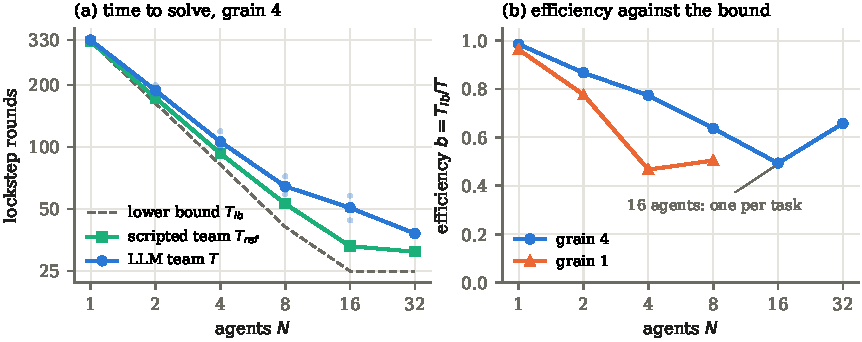
\includegraphics[width=\textwidth]{figures/scaling.pdf}
\caption{\textbf{Scaling on the 16$\times$4 problem.} (a) Rounds to solve at grain 4 (log--log). Small dots are seeds; the line is their mean. The LLM team tracks the bound up to 4 agents and then levels off above the scripted team. 32 agents are faster than 16 although both have the same bound. (b) Efficiency $b=\Tlb/T$. Coarser tasks (grain 4) scale better than fine ones (grain 1).}
\label{fig:scaling}
\end{figure*}

\subsection{Q1: Teams parallelize, but efficiency falls}

Figure~\ref{fig:scaling} and Table~\ref{tab:scaling} show the scaling curve.
A single agent is within 2\% of the bound ($b=0.98$ at grain 4, 0.96 at grain 1), which confirms that the problem leaves no room for shortcuts.
Teams do parallelize: 32 agents solve the grain-4 problem in 38 rounds, an 8.7$\times$ speed-up over one agent.
But efficiency falls with team size, to 0.64 at 8 agents and 0.49 at 16.
Coarser tasks scale better: at 8 agents, $b$ is 0.64 at grain 4 and 0.50 at grain 1, because each answer that must be shared carries more computation.

The curve is not monotone in efficiency.
At 16 and 32 agents, the bound is the span ($\Tlb=25$), and 16 agents already have one agent per task.
Yet 32 agents were faster than 16 on every seed (39, 38, 37 against 44, 58, 50).
The rest of the paper explains this.

\begin{table}[t]
\centering\small
\caption{Scaling at grain 4 ($w=16$, $d=4$), means over 3 seeds.}
\label{tab:scaling}
\begin{tabular}{@{}rrrrrr@{}}
\toprule
$N$ & $T$ & speed-up & $\Tlb$ & $\Tref$ & $b$ \\
\midrule
1 & 330.0 & 1.00 & 325 & 325 & 0.98 \\
2 & 188.0 & 1.76 & 163 & 173 & 0.87 \\
4 & 106.0 & 3.11 & 82 & 93 & 0.77 \\
8 & 64.3 & 5.13 & 41 & 53 & 0.64 \\
16 & 50.7 & 6.51 & 25 & 33 & 0.49 \\
32 & 38.0 & 8.68 & 25 & 31 & 0.66 \\
\bottomrule
\end{tabular}
\end{table}

\subsection{Q2: The time is lost at handoffs and at the join}

\begin{figure*}[t]
\centering
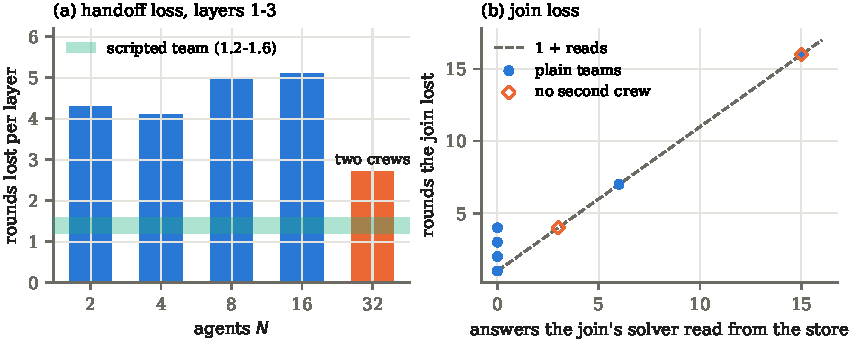
\includegraphics[width=\textwidth]{figures/losses.pdf}
\caption{\textbf{Where the time goes} (grain 4, $w=16$). (a) Mean handoff loss over layers 1--3. Teams of 2--16 lose 4--5 rounds per layer, against 1.2--1.6 for scripted teams. 32-agent teams, which split into two crews, lose 2.7. (b) Each point is one run. The join loses 1--4 rounds, plus about one round for every answer its solver reads from the store one key at a time. Diamonds are the no-second-crew intervention (\S\ref{sec:q3}).}
\label{fig:losses}
\end{figure*}

Figure~\ref{fig:losses} decomposes the gap between $T$ and the bound.
Two mechanisms account for nearly all of it.

\paragraph{Handoff.}
Up to 16 agents, each layer after the first loses 4.1--5.1 rounds on average, against 1.2--1.6 for scripted teams.
The traces show why: the agent that finishes a task and passes its answer on is also the agent that must then read the next layer's inputs and start the next task. Sharing, reading and starting are serialized in the same agent.

\paragraph{Join.}
The final task needs all 16 answers of the last layer.
When its solver gathered them from messages, the join lost 1--4 rounds.
In two of the three 16-agent runs, the solver instead read the answers from the store one key at a time, 15 and 6 reads, and the join lost 16 and 7 rounds.
Across all 18 runs, the join's loss follows one round per store read on top of a base of 1--4 rounds. The three runs with the most reads (15, 15 and 6) lost exactly reads $+1$ (Figure~\ref{fig:losses}b).

Together, these account for the gap between 16 and 32 agents. The per-layer gap is about 2.4 rounds over three layers, and the join gap is about 6 rounds, for a total of about 13 rounds against an observed 12.7.

\subsection{Q3: Spare agents form two crews}
\label{sec:q3}

The 32-agent teams split into two crews at the start of every run, without being told to: in the agents' own words, ``a0--a15 handle L0 and L2; a16--a31 handle L1 and L3''.
While one crew computes a layer, the other reads the inputs it will need and waits to start, so the handoff overlaps with computation.
Their layers lost 2.3--3.0 rounds, about half of what smaller teams lost.

\begin{figure}[t]
\centering
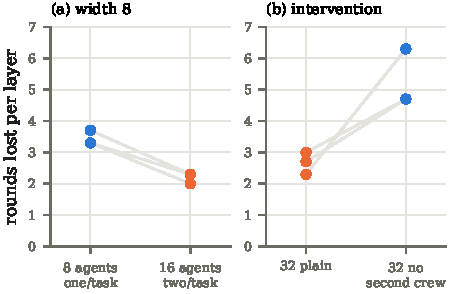
\includegraphics[width=\columnwidth]{figures/interventions.pdf}
\caption{\textbf{Two pre-registered tests of the crew mechanism}, paired by seed. (a) Out of sample, on an 8-wide problem: 16 agents (two per task) formed two crews on every seed and lost less per layer than 8 agents. (b) Intervention: forbidding the second crew in 32-agent teams raised the handoff loss on every seed.}
\label{fig:interventions}
\end{figure}

\paragraph{Out of sample.}
We predicted, before running, that on a new 8-wide problem, 16 agents (two per task) would lose less per layer than 8 agents and would be faster on every seed.
Both held on all three seeds (Figure~\ref{fig:interventions}a): 2.2 against 3.4 rounds per layer, and $T=34.7$ against 38.7.
On every seed the 16-agent teams again formed two crews, a0--a7 and a8--a15, on alternating layers.

\paragraph{Intervention.}
The association could be produced by something else that comes with having more agents.
The \texttt{peers-columns} intervention adds one rule to the 32-agent team: agent $a_K$ does column $K$ in every layer, and agents without a column take no task.
This is exactly the assignment that 16-agent teams chose for themselves, with 16 idle agents added.
The rule was obeyed throughout, and no second crew formed.
On every seed, the handoff loss rose from 2.7 to 5.2 rounds per layer (Figure~\ref{fig:interventions}b) and $T$ rose from 37--39 to 49--56, back to the level of plain 16-agent teams (44--58).
On two seeds the join's solver again read 15 answers from the store and lost 16 rounds, matching the join rule above.
\emph{Idle agents that are not allowed to form a crew buy nothing.}

\section{Pre-registered Predictions}
\label{sec:prereg}

Each prediction was committed to the repository before its runs \citep{nosek2018prereg}. Table~\ref{tab:prereg} lists all four.

\begin{table}[t]
\centering\small
\caption{All predictions, written before their runs.}
\label{tab:prereg}
\begin{tabular}{@{}p{3.9cm}p{3.3cm}@{}}
\toprule
prediction & outcome \\
\midrule
BSP: $T(32)=46$ (42--58) & failed: 38 \\
Layered BSP: $T(16)=40$ (39--50) & failed: 50.7 \\
Width 8: two per task lose less per layer, faster on every seed & held 3/3; both $\approx$3 rounds faster than predicted \\
No second crew: handoff loss $\approx$5, $T$ rises & held 3/3 \\
\bottomrule
\end{tabular}
\end{table}

\paragraph{Why the scaling laws failed.}
The BSP reading models time as $T = \text{base} + S\cdot L$, a fixed loss $L$ per superstep.
Its first base, the Brent bound, spreads the final task and each layer's remainder over the whole team, which a layer-by-layer team cannot do. That error inflated $L$.
Correcting the base after the fact still failed on the next, pre-registered size.
The USL fit came within 1 round at 32 agents, but missed 16 agents by 4.7 rounds.
Neither form can capture the result that matters most: whether a team has spare agents to form a second crew.
The mechanistic predictions, which name a cause and the traces that should show it, held every time.

\section{Discussion and Limitations}

\paragraph{What carries over.}
In any pipeline of dependent steps, an agent that both produces an output and starts the next step serializes the handoff. A team gains when some agents prepare while others compute.
LLM teams discovered this pipelining unprompted, but only when they had spare agents.
This suggests a design rule for agent systems: give a team more agents than the widest stage, or assign the second crew explicitly.

\paragraph{Limitations.}
\begin{itemize}\setlength\itemsep{1pt}
\item \textbf{One model.} All results so far come from one closed model. \todo{open-weight replication.}
\item \textbf{Three seeds.} Each setting has three seeds, and 16-agent runs vary widely (44--58 rounds). \todo{5--10 seeds for key settings.}
\item \textbf{Synthetic task.} The task is synthetic by design, so that the bound is exact. \todo{one real task with explicit dependencies.}
\item \textbf{Confounded intervention.} The intervention also changed communication: fewer messages (12--55 against 134--182) and more store reads. Its control is earlier runs rather than a concurrent randomized arm. \todo{concurrent rerun of plain 32.}
\item \textbf{Idealized time.} Lockstep rounds idealize time. \todo{asynchronous timing check.}
\end{itemize}

\section{Conclusion}
We introduced an environment where the best possible time of a team of LLM agents is known exactly, and used it to locate where the remaining time goes.
Teams scale to an 8.7$\times$ speed-up, but they lose most of their time at handoffs and at the join.
With spare agents, they recover part of it by forming crews on their own.
Pre-registered mechanistic predictions held, while curve-fitting scaling laws did not.

\paragraph{Reproducibility.}
Code, configurations, complete model-call archives, audit scripts and token accounting for every run will be released.
An interactive replay visualizes each run as a town of agents, with a live task graph and $T$ against $\Tlb$ \todo{link to anonymized demo}.

\bibliographystyle{plainnat}
\bibliography{refs}

\appendix
\section{Abandoned Versions}
\label{app:history}
\begin{itemize}\setlength\itemsep{1pt}
\item \textbf{Symbolic recurrences.} Each task was a recurrence checked by SymPy. A strong model wrote the whole DAG as one closed-form expression without calling a tool, so neither work nor span held. This motivated hidden keyed functions.
\item \textbf{Early hash version.} A grain-4 chain repeated a value and was solved in 324 actions against a bound of 325. Keys are now chosen so that no chain repeats a value.
\end{itemize}

\section{Token Usage}
\begin{table}[h]
\centering\small
\begin{tabular}{@{}lr@{}}
\toprule
experiment & tokens \\
\midrule
grain 1, $N$=1--8 & 61.3M \\
grain 4, $N$=1--8 & 149.9M \\
grain 4, $N$=32 & 90.8M \\
grain 4, $N$=16 & 59.5M \\
width 8, $N$=8, 16 & 52.7M \\
no second crew, $N$=32 & 105.9M \\
\bottomrule
\end{tabular}
\end{table}

\end{document}
